\documentclass[11pt]{article}
\usepackage[utf8]{inputenc}
\usepackage[english]{babel}
\usepackage{amssymb,amsmath,amsthm,mathtools}
\usepackage{enumitem, graphicx, hyperref}

\topmargin -0.5in
\textheight 9.0in
\oddsidemargin  -0.05in
\evensidemargin -0.05in
\textwidth 6.5in
\renewcommand
\baselinestretch{1.0}

\allowdisplaybreaks
\numberwithin{equation}{section}
 
\newcommand{\tr}{{\text{tr}}}
\newcommand{\B}[1]{\textbf{#1}}
\newcommand{\T}[1]{\texttt{#1}}

\title{Picturing quantum state space}
\author{Matthew B. Weiss}
\date{\today}

\begin{document}
\maketitle 

In casting about for ideas for our final figure, I returned to an idea I mentioned earlier, that of measuring the so-called triple products $\tr(\sigma_i \sigma_j \sigma_k)$ where $\{\sigma_i\}$ may be regarded as SIC states, or any IC WH-POVM states, or really any set of IC states you like, although we'll specialize to the former. As we all by now well know, QBists view quantum theory as probability theory with the addition of nonclassical coherence contraints, e.g.,
\begin{align}
P(E) = \sum_{ij} P(E|R_i)\Phi_{ij} P(R_j),
\end{align}
where $P(R_j)$ are probabilities with respect to the reference measurement which characterize some state $\rho$, $P(E|R_i)$ are conditional probabilities which characterize some effect $E$, and $\Phi=P(R|R)^{-1}$ in the case we care about. But there is more to the story. Quantum theory puts specific constraints on the probabilities $P(R_j)$ which one can consistently assign to the reference measurement. The set of ``valid'' probability distributions forms a special subset of the probability simplex which correspond to density matrices. Probability distributions outside this subset correspond to Hermitian matrices with negative eigenvalues (!). So how can we characterize the set of valid distributions, that is, the shape of quantum state space? For QBists, it is all about consistency. 

Consider the following circuit from the very nice paper, ``Measuring relational information between quantum states, and applications,''\footnote{https://arxiv.org/abs/2109.10006}
\begin{center}
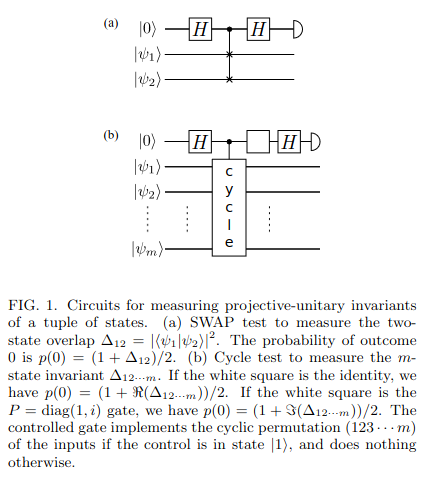
\includegraphics[scale=0.5]{rel.png}
\end{center}
It gives us a nice recipe. Prepare a qubit in the $|0\rangle$ state alongside a triple of states $\sigma_i, \sigma_j, \sigma_k$. We first apply a Hadamard to the qubit, followed by a cyclic shift of the triple of states, coherently controlled by the state of the qubit. Finally, we Hadamard the qubit, and measure it. One can show that $P(0) = \frac{1}{2}(1 + \Re[\tr(\sigma_i \sigma_j \sigma_k)])$. In other words, one can extract the real part of the triple product $\tr(\sigma_i \sigma_j \sigma_k)$ directly from this outcome probability. (The recipe works for any $n$-product, and the imaginary part can be extracted too. Buzzword: it is a generalized swap trick.) Let $R_{ijk} = \Re[\tr(\sigma_i \sigma_j \sigma_k)]$. This will be a symmetric tensor so we of course don't need to measure all possible triples. Specializing to the case where we have $d^2$ states, e.g., SIC states, $R$ will be a $(d^2, d^2, d^2)$ tensor.  For $d=2$,  it can be obtained by running 20 circuits. For $d=4$, 816 circuits. Let us now show how the shape of quantum state space can be characterized in terms of consistency with the results of running these circuits.

\begin{figure}[t]
    \centering
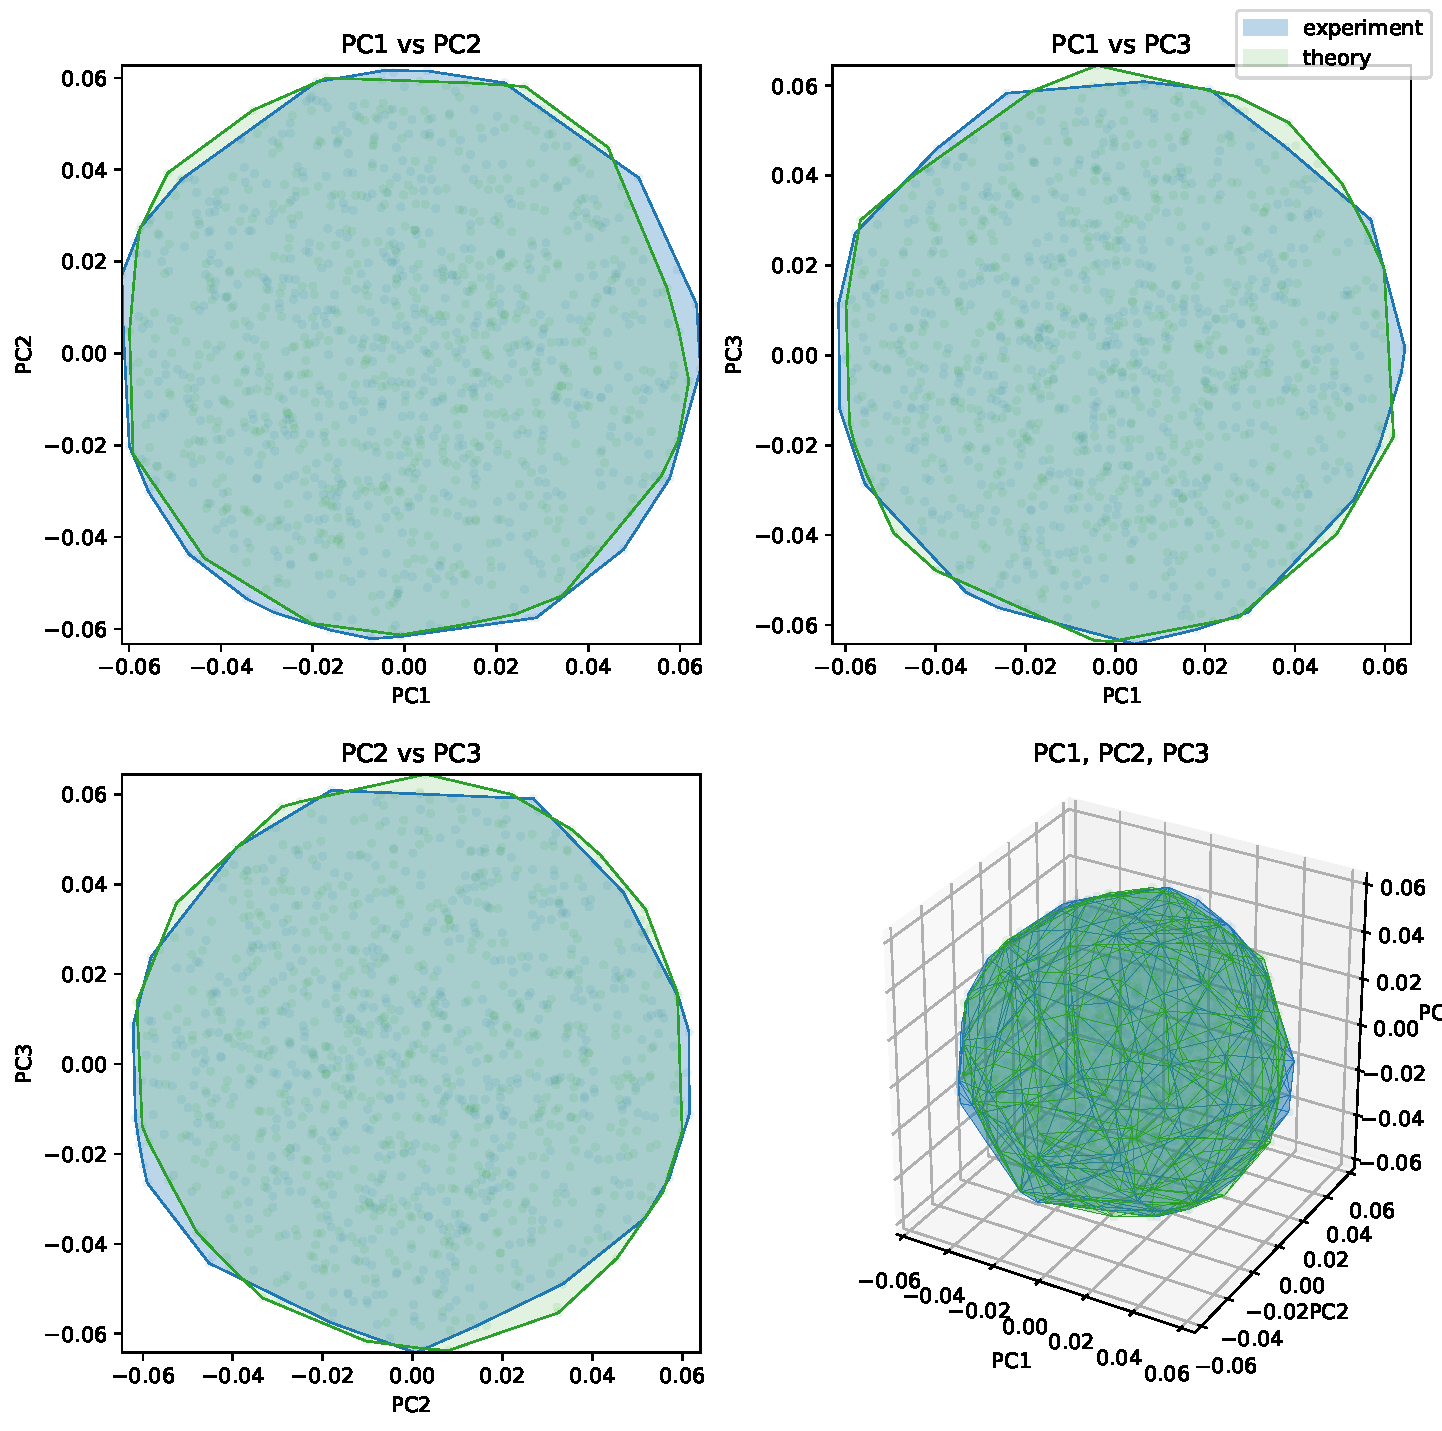
\includegraphics[scale=0.5]{triples_d2.pdf}  
    \caption{$d=2$ state space reconstruction. ``Experiment'' here means I used only 500 shots in the triple product circuits with no noise model.}
    \label{fig:d2}
\end{figure}


First, we define a matrix $L_{P(R)}$ corresponding to a distribution $P(R)$,
\begin{align}
[L_{P(R)}]_{ij} = \sum_{kl} R_{ijk}\Phi_{kl} P(R_l) = \sum_{kl} \Re[\tr(\sigma_i \sigma_j \sigma_k)]\Phi_{kl}P(R_l) = \Re[\tr(\sigma_i \sigma_j \rho)],
\end{align}
where we've used the reconstruction formula $\rho = \sum_{kl}\Phi_{kl}P(R_l)\sigma_k$. But then
\begin{align}
\sum_{ij} x_i [L_{P(R)}]_{ij} x_j &= \sum_i x_i\tr(\sigma_i \sigma_j \rho)x_j + \sum_i x_i\tr(\sigma_i \rho \sigma_j)x_j=2 \tr(X^2 \rho),
\end{align}
where $X = \sum_i x_i \sigma_i$. Since the states $\{\sigma_i\}$ are informationally complete, and the $x$'s are real valued, we can obtain any and all Hermitian operators $X$ this way. Clearly, $X^2$ must be positive semidefinite, and so $\tr(X^2 \rho) \ge 0$ iff $\rho$ itself is positive semidefinite. But we have just shown that this is equivalent to $\sum_{ij} x_i [L_{P(R)}]_{ij} x_j \ge 0$, in other words, $L_{P(R)} \ge 0$ is positive semidefinite itself. In other words, a probability distribution $P(R)$ on reference outcomes is valid (corresponds to a quantum state) iff $L_{P(R)} \ge 0$: moreover, one can calculate $L_{P(R)}$ in terms of the fundamental tensor $R$, whose entries are built out of the probabilities we assign to the outcomes of the aforementioned generalized swap trick circuits. Thus consistency with all of $d$-dimensional quantum mechanics amounts to consistency, properly understood, with the triple product experiments on the reference states $\{\sigma_i\}$.

\begin{figure}[b]
    \centering

\includegraphics[scale=0.4]{triples_d4.pdf}  
    \caption{$d=4$ state space reconstruction. Again just 500 shots per circuit.}
    \label{fig:d4}
\end{figure}


I have already added code to generate the triple product circuits to the repository. The proposal for the final figure is the following: to construct the tensor $R$ empirically, and then use it to ``reconstruct'' the state space, comparing it to theory. In the simplest case, one can randomly sample probability distributions $P(R)$ uniformly in the simplex, keeping only those for which $L_{P(R)} \ge 0$, and thus develop an image of the effective state space according to this criterion of consistency. We can then compare this image to the ``true'' state space, for comparison obtained the same way, by sampling distributions and keeping only those marked as valid by the theoretical tensor $R$. For $d=2$, the probability distributions are 4-dimensional, and can be projected into 3D in order to be visualized: see Figure \ref{fig:d2}. For $d=4$, we can try to visualize the overlap between the empirical and theoretical state spaces by projecting into two and three dimensions in a variety of ways: Figure \ref{fig:d4}. Quantitatively, one could calculate the overlap between the theoretical and empirical state spaces, what proportion of the former is contained in the latter, and vice versa: it would be interesting to come up with additional measures for how close we get.

There are some technical challenges here: as the dimension grows, the proportion of the simplex taken up by the valid states diminishes quickly, and so it is difficult to build up a good picture by naive sampling. Since states near the center of the simplex are generally valid, I try to sample from the center of the simplex outward. But of course, this loses detail up near the boundary of the state space: you can see in Figure \ref{fig:d4} that even the ``theoretical'' result looks pretty bad. On the one hand, rather the sampling I could try to ``solve'' directly for valid solutions. On the other hand, one can characterize the boundary states using a scalar equation also related to the tensor $R$: we could instead focus our attention there. I'll continue to experiment with different ways of making this type of visualizion effective. Finally, on the theory side, it would be interesting to relate anomalies in the state space reconstruction to different types of hardware errors. 


\end{document}
